%%%%%%%%%%%%%%%%%%%%%%%%%%%%%%
\section{La chaîne de pendule}
%%%%%%%%%%%%%%%%%%%%%%%%%%%%%%

\subsection{Le pendule pesant}
\begin{multicols}{2}%\columnbreak\end{multicols}
\begin{tikzpicture}
%\draw [ball color=gray] (0,0)coordinate(A)node[left]{$m$\ \ \ } circle (.3);
\draw [ball color=gray] (0,0)coordinate(A)node[below=3mm]{$m$} circle (.3);
\draw (0.21,0.21) -- (45:4.7)coordinate(B)node[right]{O}node[pos=.5,left=2mm]{$l$};
%\draw (0,0)coordinate(A)node[left]{m}circle(.1)-- (40:5)coordinate(B)node[right]{O};=3mm
\draw[dashed](B)--++(0,-5)coordinate(C);
\draw pic[ draw ,<->,"$\theta$",angle eccentricity =1.5, angle radius=1cm]{ angle =A--B--C};
%\draw[dotted,thick](0,0)arc(-135:-90:5);node[right]{B}
\draw [->](5,2) --++(0,-2)node[pos=.5,left]{$\overrightarrow{g}$};
\end{tikzpicture}

\columnbreak
Un pendule pesant est constitué par une masse $m$ suspendue à un fil rigide de longueur $l$ relié à un point O. Une liaison en ce point permet au pendule de tourner autour d'un axe fixe. L'angle entre le fil et la verticale est noté $\theta$. La masse est soumise à son poids $\overrightarrow{P}=m\overrightarrow{g}$, à la réaction du fil $\overrightarrow{R}$ et à une force de frottement visqueux $\overrightarrow{f}= - \frac{\beta}{l} \overrightarrow{v}$. La relation fondamentale de la dynamique donne :
\[
m l\ \frac{d^2 \theta}{\dt^2} =  - m g \sin{\theta}  -  \beta\ \frac{d \theta}{\dt}
\]
\end{multicols}
%
\subsection{Les pendules couplés}
\begin{multicols}{2}%\columnbreak\end{multicols}
Deux pendules pesants sont reliés par un fil de torsion suivant leur axe fixe commun.  La relation fondamentale de la dynamique donne alors :
\[\left\{
  \begin{array}{rcr}
m l\ \frac{d^2 \theta _1}{\dt^2} & = &  - m g \sin{\theta _1}  -  \beta\ \frac{d \theta _1}{\dt} - kl (\theta _1 - \theta _2) \\
m l\ \frac{d^2 \theta _2}{\dt^2} & = &  - m g \sin{\theta _2}  -  \beta\ \frac{d \theta _2}{\dt} - kl (\theta _2 - \theta _1) \\
  \end{array}
\right.\]
dans le cas où les pendules sont identiques.

\columnbreak
\begin{tikzpicture}
\draw [ball color=gray] (0,0)coordinate(A)node[below=3mm]{$m$} circle (.2);
\draw (0.13,0.13) -- (65:2.7)coordinate(B);%node[right]{O}node[pos=.5,left=2mm]{$l$};
\draw[dashed](B)--++(0,-3)coordinate(C);
\draw pic[ draw ,<->,"$\theta _1$",angle eccentricity =1.5, angle radius=1cm]{ angle =A--B--C};
%
\draw [ball color=gray] (3,0.3)coordinate(D)node[below=3mm]{$m$} circle (.2);
\draw (3.13,0.43) -- (35:5.1)coordinate(E);%node[right]{O}node[pos=.5,left=2mm]{$l$};
\draw[dashed](E)--++(0,-3)coordinate(F);
\draw pic[ draw ,<->,"$\theta _2$",angle eccentricity =1.5, angle radius=1cm]{ angle =D--E--F};
%
\draw[decorate,decoration={coil,segment length=10pt,amplitude=0.2cm,aspect=.8}](B)--(E)node[pos=.5,above=2mm]{$k$};
\end{tikzpicture}
\end{multicols}
%
%
%
\subsection{La chaîne de pendule}
Une chaîne de pendule est constituée d'une série de pendules pesants. Chaque pendule étant couplé avec ses deux plus proches voisins à l'aide d'un fil de torsion.

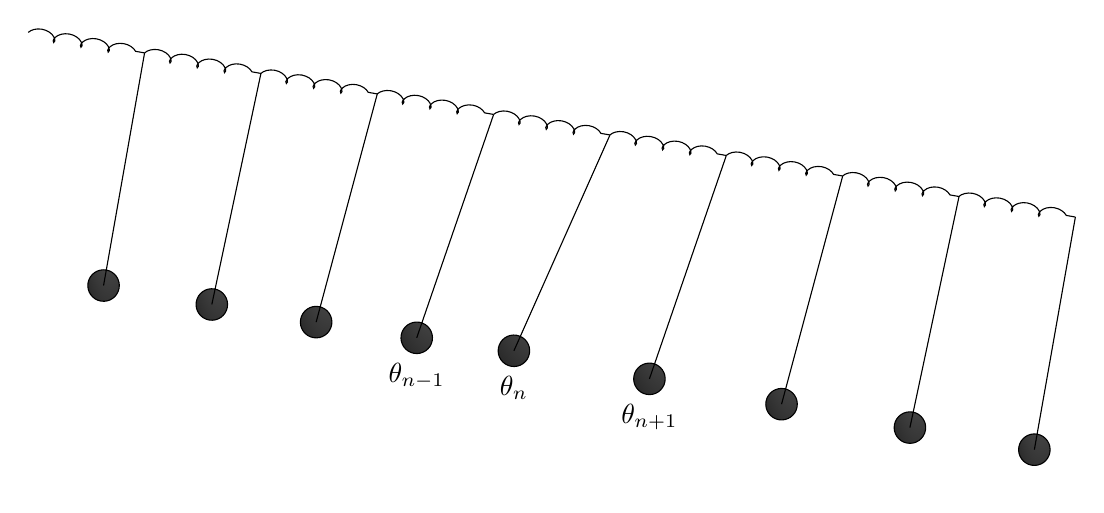
\begin{tikzpicture}[rotate=-10]
\foreach \x/\t/\a in {1/{}/0, 2/{}/2, 3/{}/5, 4/{\theta _{n-1}}/9, 5/{\theta _n}/14, 6/{\theta _{n+1}}/9, 7/{}/5, 8/{}/2, 9/{}/0}
{
\coordinate (A) at (1.5*\x,0) ;
\draw[decorate,decoration={coil,amplitude=0.07cm,aspect=1.1}](A)-- ++(1.5,0)coordinate(B);
\draw (B) -- ++(-90-\a:3)[ball color=gray] ++(0,0) circle (.2) node[below=2mm]{$\t$};
%\draw;
}
\end{tikzpicture}

\label{chaineDePendule}
\subsection{L'équation de la chaine de pendule}
La chaîne de pendule est constituée d'une série de pendules pesants. Chaque pendule étant couplé avec ses deux plus proches voisins à l'aide d'un fil de torsion.\cite{sine-gordon}\cite{chaine-pendule}
\[
\frac{\mathrm d^2\theta _n}{\mathrm d t^2} - c^2 \frac{\theta _{n+1} + \theta _{n-1} - 2 \theta _n}{\mathrm{a} ^2} + \omega _0 ^2 \sin \theta _n = 0
\]
%
\begin{center}
\begin{tabular}{cccc}
%\multicolumn{4}{|c|}{Contrôles} & \multicolumn{4}{c}{Information} & \multicolumn{4}{|c|}{Contrôles}\\
$\frac{k}{m}$ & $\frac{vitesse^2}{longueur^2}$ & T$^{-2}$ & $\frac{k}{m}$ = $\frac{c^2}{a^2}$ \\
$\frac{g}{l}$& pulsation$^2$ & T$^{-2}$ & $\frac{g}{l}$ = $\omega _0 ^2$ \\
\end{tabular}
\end{center}

La relation fondamentale de la dynamique, donne, en prennant en compte les frottements visqueux :
\[
m l\ \frac{d^2 \theta _n}{\dt^2} =  - m g \sin{\theta _n}  -  k l \Delta \theta _n(t)  -  \beta\ \frac{d \theta _n}{\dt}
\]
soit
\[
\frac{d^2 \theta _n}{\dt^2} =  - \frac{g}{l} \sin{\theta _n}  -  \frac{k}{m} \Delta \theta _n(t)  - \frac{\beta}{ml}\ \frac{d \theta _n}{\dt}
\]
avec
\begin{center}
\begin{tabular}{cccccc}
 & {\it abréviation} & {\it grandeur} & {\it dimension} &  \\
 & $\theta _n$ & angle & radian &  \\
 & m & masse & M &  \\
 & g & pesanteur & LT$^{-2}$ &  \\
 & k & torsion & MT$^{-2}$ &  \\
 & l & longueur & L &  \\
 & $\beta$ & frottement & ML$^{2}$T$^{-1}$ &  \\
\end{tabular}
\end{center}
%
\subsection{Expressions des forces et des énergies associées}

La force de rappel, s'exerçant sur la masse m, dû au fil de torsion entre les pendules est :
\[
f_{torsion} = -  k l \Delta \theta _n = -  k l\ (2\theta _n-\theta _{n-1}-\theta _{n+1})
\]
L'énergie potentielle entre les pendules n et n-1 est :
\[
E_{couplage} = \frac{1}{2}\ k l^2 (\theta _n-\theta _{n-1})^2
\]

La force de rappel dû à la gravitation est :
\[
f_{gravitation} = - m g \sin{\theta _n}
\]
L'énergie potentielle de pesanteur de la masse m est :
\[
E_{pp} = m g l (1 - \cos{\theta _n})
\]
La linéarisation de cette dernière force donne lieu à une force de rappel harmonique :
\[
f_{ressort} = - m g \theta _n
\]
L'énergie potentielle correspondante est alors:
\[
E_{pp} = \frac{1}{2}\ m g l \theta _n^2
\]

Enfin, l'énergie cinétique découle du travail de 
\[
m l\ \frac{d^2 \theta _n}{\dt^2}
\]
%
Et vaut
\[
E_{c} = \frac{1}{2}\ m l (\frac{d \theta _n}{\dt})^2
\]


La force de frottement visqueux est :
%
\[
f_{frottement} = -  \beta\ \frac{\theta _n(t) - \theta _n(t-\dt)}{\dt}
\]
%
La présence de cette force implique une dissipation de l'énergie. En l'absence de cette force, on doit observer une conservation de l'énergie totale.

À ces forces il faut ajouter le courant josephson, correspondant à une constante additive dans la relation fondamentale de la dynamique ainsi que la force s'exerçant sur le premier pendule lors de l'excitation de la chaîne.
%%%%%%%%%%%%%%%%%%%%%%%%%%%%%%%%%%%%%%%%%%%%%%%%%%%%%%%%%%%%%%%%%
%La relation fondamentale de la dynamique donne :
%\[- m g \sin{\theta _n(t)}  -  k l \Delta \theta _n(t)  -  \beta\ \frac{\theta _n(t) - \theta _n(t-\dt)}{\dt} =  m l\ \frac{\theta _n(t+\dt) - 2\theta _n(t) + \theta _n(t-\dt)}{\dt^2}\]
%soit\[\frac{\theta _n(t+\dt) - 2\theta _n(t) + \theta _n(t-\dt)}{\dt^2} = - \frac{g}{l} \sin{\theta _n(t)}  -  \frac{k}{m} \Delta \theta _n(t)  -  \frac{\beta}{ml}\ \frac{\theta _n(t) - \theta _n(t-\dt)}{\dt}\]
%D'ou finallement\[\theta _n(t+\dt) = 2\theta _n(t) - \theta _n(t-\dt) + \delta force_n\]
%avec \[\delta force_n = - \dt^2 \frac{g}{l} \sin{\theta _n(t)} - \dt^2 \frac{k}{m} \Delta \theta _n(t) - \dt \frac{\beta}{ml} (\theta _n(t) - \theta _n(t-\dt))\]
%%%%%%%%%%%%%%%%%%%%%%%%%%%%%%%%%%%%%%%%%%%%%%%%%%%%%%%%%%%%%%%%%
\subsection{Résumé des forces et des énergies}
\begin{center}
\begin{tabular}{ccc}
%\multicolumn{4}{|c|}{Contrôles} & \multicolumn{4}{c}{Information} & \multicolumn{4}{|c|}{Contrôles}\\
 & force & énergie \\
torsion & -  k l $\Delta \theta _n$ & $\frac{1}{2}$ k l$^2 (\theta _n-\theta _{n-1})^2$ \\
gravitation & - m g $\sin{\theta _n}$ & m g l (1 - $\cos{\theta _n}$) \\
harmonique & - m g $\theta _n$ & $\frac{1}{2}$ m g l $\theta _n^2$ \\
inertie & m l $\frac{d^2 \theta _n}{\dt^2}$ & $\frac{1}{2}$ m l$^2$ $(\frac{d \theta _n}{\dt})^2$ \\
courant & josephson & \\
\end{tabular}
\end{center}
%
